% !TEX TS-program = XeLaTeX
% Commands for running this example:
% 	 xelatex Xindy_Make_Index
%     xindy -L persian -C utf8 -M texindy Xindy_Make_Index.idx
% End of Commands
\documentclass[a4paper]{article}
\pagestyle{empty}
\usepackage{graphicx}
\usepackage[colorlinks]{hyperref}
\usepackage{makeidx}
\makeindex
\usepackage{xepersian}

\begin{document}
\عنوان{ساخت نمایه با   \lr{Xindy Make Index} }
\نویسنده{\url{http://forum.parsilatex.com/}}
\تاریخ{}
\عنوان‌ساز
\شروع{شمارش}
\فقره 
دستور 
\verb|\usepackege{mekeidx}|
 قبل از  فراخوانی بسته‌ی \XePersian قرار دهید.
\فقره
کلمات مورد نظر خود مثلا \lr{word} با دستور \verb|\index{word}| ایندکس کنید.
\فقره
نحوه‌ی اجرای \lr{Make Index}   در ویرایشگرهای \lr{TeX Maker} و \lr{TeX Works}:
\شروع{فقرات}
\فقره  تک‌میکر: از منوی \lr{Tools} گزینه‌ی \lr{Xindy Make Index} را کلیک کنید یا از دکمه‌‌های میانبر \lr{Ctrl+Alt+I} استفاده کنید.

\فقره  تک‌ورکز: ابتدا باید مثل عکس زیر تنظیم  و سپس گزینه‌ی \lr{Xindy Make Index}  انتخاب و روی دکمه‌ی سبز رنگ کلیک کنید یا از دکمه‌های  \lr{Ctrl+T} استفاده کنید.

\begin{figure}[!h]
\centerline{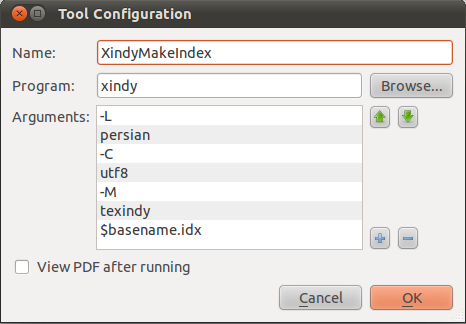
\includegraphics[width=\textwidth]{Xindy_Make_Index.png}}
\end{figure}

\پایان{فقرات}
 \پایان{شمارش}




\index{کتاب}
\index{پارسی‌لاتک}
\index{بی‌دی}
\index{سوال}
\index{عنصر}
\index{گزینه}
\index{ژاکت}
\index{مرکز دانلود}
\index{اجرا}
\index{تک‌لایو}
\index{ثالث}
\index{جهان}
\index{چهار}
\index{حمایت}
\index{خواهش}
\index{دنیا}
\index{زی‌پرشین}
\index{ریحان}
\index{شیرین}
\index{صمیمی}
\index{ضمیر}
\index{طبیب}
\index{ظاهر}
\index{غریب}
\index{قوی}
\index{لاتک}
\index{نان}
\index{وحید}
\index{همه}
\index{یک}

\printindex
\end{document}